% ===================================================================
%  Week 9 — Contours, Components & Shape Analysis
% ===================================================================
\documentclass[10pt,aspectratio=169]{beamer}
% ===================================================================
%  Shared Beamer preamble for "Practical Image Processing"
%  English slides. Compile with pdfLaTeX.
% ===================================================================

\usetheme{metropolis}
\usepackage[T1]{fontenc}
\usepackage[utf8]{inputenc}
\usepackage{lmodern}
\usepackage{listings}
\usepackage{tcolorbox}
\usepackage{fontawesome5}
\usepackage{booktabs}
\usepackage{amsmath,amssymb}
\usepackage{tikz}
\usepackage{pgfplots}
\pgfplotsset{compat=1.17}
\usetikzlibrary{arrows.meta,positioning,shapes.geometric,fit,backgrounds,matrix}
\tcbuselibrary{skins,breakable}

% ---- Palette --------------------------------------------------------
\definecolor{coursePrimary}{HTML}{1B4965}   % deep blue
\definecolor{courseAccent}{HTML}{E76F51}    % coral
\definecolor{courseGood}{HTML}{2A9D8F}      % teal
\definecolor{courseBad}{HTML}{C0392B}       % red
\definecolor{courseInfo}{HTML}{2980B9}      % blue
\definecolor{codeBg}{HTML}{F5F6FA}
\definecolor{codeKw}{HTML}{8E44AD}
\definecolor{codeStr}{HTML}{2A9D8F}
\definecolor{codeCom}{HTML}{7F8C8D}

\setbeamercolor{frametitle}{bg=coursePrimary}
\setbeamercolor{progress bar}{fg=courseAccent}
\setbeamercolor{alerted text}{fg=courseAccent}
\metroset{block=fill,sectionpage=progressbar,numbering=fraction}

% ---- Code listings (Python is built into listings) -----------------
\lstdefinestyle{course}{
  backgroundcolor=\color{codeBg},
  basicstyle=\ttfamily\scriptsize,
  keywordstyle=\color{codeKw}\bfseries,
  stringstyle=\color{codeStr},
  commentstyle=\color{codeCom}\itshape,
  numberstyle=\tiny\color{codeCom},
  numbers=left, numbersep=6pt,
  showstringspaces=false, breaklines=true, breakatwhitespace=true,
  tabsize=4, columns=fullflexible,
  frame=single, framesep=4pt, rulecolor=\color{gray!30},
  keepspaces=true, upquote=true, language=Python,
}
\lstset{style=course}
\lstdefinelanguage{bash}{
  keywords={cd,pip,python,venv,source,import}, sensitive=true,
  morecomment=[l]{\#}, morestring=[b]', morestring=[b]",
}

% ---- Reusable callout boxes ----------------------------------------
\newtcolorbox{goodbox}[1][Good practice]{colback=courseGood!8,colframe=courseGood,
  fonttitle=\bfseries,title={\faCheck~#1},boxrule=0.6pt,left=4pt,right=4pt,top=3pt,bottom=3pt}
\newtcolorbox{badbox}[1][Pitfall]{colback=courseBad!8,colframe=courseBad,
  fonttitle=\bfseries,title={\faTimes~#1},boxrule=0.6pt,left=4pt,right=4pt,top=3pt,bottom=3pt}
\newtcolorbox{infobox}[1][Note]{colback=courseInfo!8,colframe=courseInfo,
  fonttitle=\bfseries,title={\faInfoCircle~#1},boxrule=0.6pt,left=4pt,right=4pt,top=3pt,bottom=3pt}
\newtcolorbox{mathbox}[1][Math]{colback=coursePrimary!6,colframe=coursePrimary,
  fonttitle=\bfseries,title={\faCalculator~#1},boxrule=0.6pt,left=4pt,right=4pt,top=3pt,bottom=3pt}

\newcommand{\keyidea}[1]{\begin{alertblock}{Key idea}#1\end{alertblock}}
\newcommand{\term}[1]{\textbf{\color{coursePrimary}#1}}
\newcommand{\code}[1]{\lstinline[basicstyle=\ttfamily\small]|#1|}

% ---- A helper to draw a small pixel grid, cells shaded by value ----
% \pixelgrid{ {10,20,120,200,240}, {30,60,130,180,230}, ... }
\newcommand{\pixelgrid}[1]{%
  \begin{tikzpicture}[font=\scriptsize,scale=0.6]
    \foreach \row [count=\ry] in {#1} {
      \foreach \val [count=\cx] in \row {
        \draw[gray,fill=coursePrimary!8] (\cx,-\ry) rectangle ++(1,-1);
        \node at (\cx+0.5,-\ry-0.5) {\val};
      }
    }
  \end{tikzpicture}}


\title{Contours \& Shape Analysis}
\subtitle{Week 9 — From regions to measurable objects}
\author{Practical Image Processing}
\date{Lecture 9 \textbullet\ 60--70 min}

\begin{document}

\maketitle

\begin{frame}{Recap \& today}
  \begin{columns}[T]
    \begin{column}{0.58\textwidth}
      \begin{itemize}
        \item Wk8: segmentation gives separated regions/blobs.
        \item \alert{Today:} \term{contours} — the outlines of those regions — and how to
              \term{measure} shape: area, perimeter, bounding box, and shape descriptors.
      \end{itemize}
    \end{column}
    \begin{column}{0.42\textwidth}
      \begin{alertblock}{DocScan milestone}
        Find each digit's contour, crop it by its bounding box, and order the digits — the last
        step before reading (Week 13).
      \end{alertblock}
    \end{column}
  \end{columns}
\end{frame}

\begin{frame}{Roadmap}\tableofcontents\end{frame}

% ==================================================================
\section{Finding contours}
% ==================================================================

\begin{frame}{A contour = the outline of a region}
  \begin{columns}[T]
    \begin{column}{0.5\textwidth}\begin{center}
      
\includegraphics[width=0.95\linewidth]{../assets/binary.png}\\{\scriptsize binary digits}\\[4pt]
      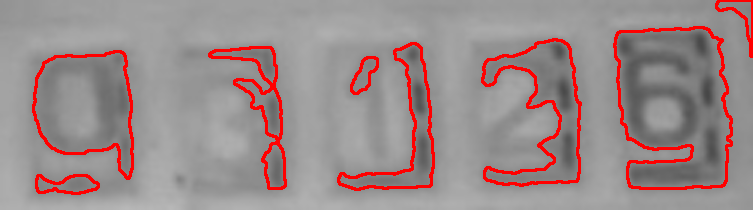
\includegraphics[width=0.95\linewidth]{../assets/contours.png}\\{\scriptsize contours (red)}
    \end{center}\end{column}
    \begin{column}{0.5\textwidth}
      \begin{itemize}
        \item A \term{contour} is an ordered list of boundary points of a connected white region.
        \item From a clean binary image, \code{findContours} traces each object's outline.
        \item Each contour is one object you can measure and crop.
      \end{itemize}
    \end{column}
  \end{columns}
\end{frame}

\begin{frame}[fragile]{findContours: modes \& approximation}
\begin{lstlisting}[language=Python]
contours, hierarchy = cv2.findContours(binary,
    cv2.RETR_EXTERNAL,        # only outer contours (ignore holes)
    cv2.CHAIN_APPROX_SIMPLE)  # compress straight segments to endpoints
\end{lstlisting}
  \begin{itemize}
    \item \term{RETR\_EXTERNAL}: outer boundaries only. \term{RETR\_TREE}: full nesting hierarchy.
    \item \term{CHAIN\_APPROX\_SIMPLE}: stores only corner points (a rectangle = 4 points, not hundreds).
  \end{itemize}
\end{frame}

\begin{frame}{Contours vs connected components}
  \begin{itemize}
    \item \term{Connected components} label each pixel with its region id (a labelled image).
    \item \term{Contours} give the ordered \emph{boundary} of each region (a list of points).
    \item Use components to count/label; contours to measure shape and crop. Often used together.
  \end{itemize}
  \keyidea{Both turn a binary mask into a list of objects — the bridge from pixels to countable, measurable things.}
\end{frame}

% ==================================================================
\section{Measuring shape}
% ==================================================================

\begin{frame}{Basic measurements}
  \begin{center}
  \begin{tabular}{@{}ll@{}}
    \toprule
    \textbf{Measurement} & \textbf{OpenCV} \\
    \midrule
    Area & \code{cv2.contourArea(c)} \\
    Perimeter & \code{cv2.arcLength(c, True)} \\
    Bounding box (axis-aligned) & \code{cv2.boundingRect(c)} \\
    Rotated box & \code{cv2.minAreaRect(c)} \\
    Enclosing circle & \code{cv2.minEnclosingCircle(c)} \\
    Centroid & from \code{cv2.moments(c)} \\
    \bottomrule
  \end{tabular}
  \end{center}
  These turn a shape into numbers you can filter, sort, and compare.
\end{frame}

\begin{frame}{Bounding boxes $\rightarrow$ crop \& order the digits}
  \begin{center}
  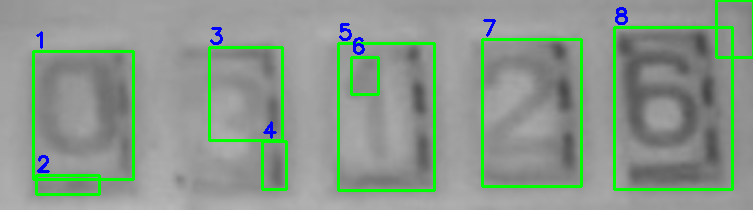
\includegraphics[width=0.85\linewidth]{../assets/boxes.png}
  \end{center}
  \begin{itemize}
    \item Draw a box around each digit; sort boxes by their $x$-coordinate (left to right).
    \item Crop each box $\rightarrow$ one clean image per digit, \emph{in order}.
    \item This is exactly the DocScan hand-off to the recognizer (Week 13).
  \end{itemize}
\end{frame}

\begin{frame}{Filtering by shape}
  \begin{itemize}
    \item Real images give junk contours (noise specks, partial marks). Filter them out by:
    \item \term{Area} (too small = noise), \term{aspect ratio} (digits are taller than wide), \term{extent} (fill fraction).
    \item Keep only contours that look like digits — a few thresholds remove most false positives.
  \end{itemize}
  \begin{goodbox}
    ``Keep contours with area $>$ T and 0.2 $<$ w/h $<$ 1.0'' filters noise from digits robustly.
  \end{goodbox}
\end{frame}

\begin{frame}{Convex hull \& convexity}
  \begin{columns}[T]
    \begin{column}{0.5\textwidth}\begin{center}
      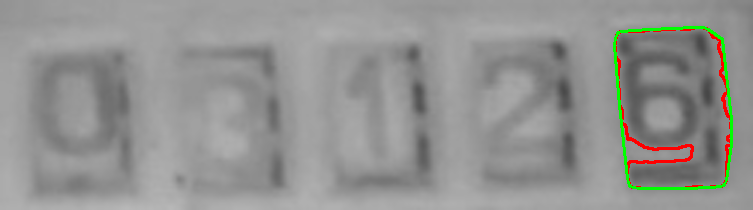
\includegraphics[width=0.95\linewidth]{../assets/hull.png}\\{\scriptsize contour (red) + convex hull (green)}
    \end{center}\end{column}
    \begin{column}{0.5\textwidth}
      \begin{itemize}
        \item \term{Convex hull}: the smallest convex shape enclosing the contour (a rubber band).
        \item \term{Convexity defects} (dents) reveal fingers, gaps, or touching-object necks.
        \item \term{Solidity} = area / hull area — how ``filled'' a shape is.
      \end{itemize}
    \end{column}
  \end{columns}
\end{frame}

% ==================================================================
\section{Shape descriptors}
% ==================================================================

\begin{frame}{Descriptors: numbers that describe a shape}
  \begin{itemize}
    \item \term{Circularity} $= 4\pi\,\mathrm{area}/\mathrm{perimeter}^2$ (1 for a circle, lower for complex shapes).
    \item \term{Aspect ratio}, \term{extent} (area/box area), \term{solidity} (area/hull area).
    \item \term{Moments}: weighted sums that summarize a shape (centroid, orientation, spread).
  \end{itemize}
  \begin{mathbox}
    Centroid: $\bar{x}=M_{10}/M_{00}$, $\bar{y}=M_{01}/M_{00}$, where $M_{00}$ is the area.
  \end{mathbox}
\end{frame}

\begin{frame}{Hu moments: rotation/scale-invariant shape}
  \begin{itemize}
    \item \term{Hu moments}: 7 numbers that are (nearly) invariant to \term{translation, rotation, and scale}.
    \item So the same shape gives the same descriptor regardless of where/how big/rotated it is.
    \item Useful for matching a shape to a template — a classical alternative to a neural net.
  \end{itemize}
  \begin{goodbox}
    \code{cv2.matchShapes} compares two contours via Hu moments — a quick shape similarity score.
  \end{goodbox}
\end{frame}

\begin{frame}{Contour approximation (polygon fitting)}
  \begin{itemize}
    \item \code{approxPolyDP} simplifies a contour to fewer points within a tolerance.
    \item A page/document boundary $\rightarrow$ approximates to \emph{4 points} = the corners.
    \item Those 4 corners feed the perspective correction in Week 11 — the DocScan ``flatten'' step.
  \end{itemize}
  \keyidea{Approximating the page contour to a quadrilateral is how DocScan finds the page's corners.}
\end{frame}

\begin{frame}{Contour hierarchy (holes)}
  \begin{itemize}
    \item \term{RETR\_TREE} returns a hierarchy: which contour is inside which (a digit ``0'' has an outer and an inner contour).
    \item Useful to count holes (a ``0'' and ``8'' have them; a ``1'' doesn't) — a cheap feature.
    \item For simple digit cropping, \term{RETR\_EXTERNAL} (outer only) is usually enough.
  \end{itemize}
\end{frame}

% ==================================================================
\section{In-class exercise}
% ==================================================================

\begin{frame}{\faPen~In-class exercise (12 min)}
  \begin{infobox}[Design the filter]
  \end{infobox}
  You have contours from a meter photo: 9 digits plus some noise specks and a long scratch.
  \begin{enumerate}
    \item Which measurements distinguish a digit from a speck? From a scratch?
    \item Write a filter rule (area + aspect ratio) that keeps digits and drops the rest.
    \item After filtering, how do you output the number in the correct order?
  \end{enumerate}
\end{frame}

\begin{frame}{\faPen~Debrief}
  \begin{itemize}
    \item Speck: tiny area $\rightarrow$ drop by \code{area > T}. Scratch: extreme aspect ratio (very wide/thin) $\rightarrow$ drop.
    \item Rule: keep if \code{area>200 and 0.2<w/h<1.2} — digits are compact and tallish.
    \item Order: sort the kept bounding boxes by $x$; read left to right.
  \end{itemize}
  \keyidea{Shape measurements turn ``which blobs are digits?'' into a few numeric thresholds.}
\end{frame}

% ==================================================================
\section{Deep dive}
% ==================================================================

\begin{frame}{Counting \& measuring objects}
  \begin{itemize}
    \item Count = number of valid contours (after filtering) — cells, coins, parts, digits.
    \item Measure = area/length/diameter per contour, converted to real units via a known scale.
    \item This is the backbone of industrial inspection and microscopy — pure classical vision.
  \end{itemize}
  \begin{goodbox}
    A calibrated pixel-to-mm ratio turns contour measurements into real-world dimensions.
  \end{goodbox}
\end{frame}

\begin{frame}{Robustness: the real-world contour mess}
  \begin{itemize}
    \item Contours are only as good as the binary mask — garbage in, garbage out.
    \item Broken digit $\rightarrow$ two contours; merged digits $\rightarrow$ one. Fix upstream (Weeks 7--8).
    \item Always filter by shape \emph{and} sanity-check the count on real data.
  \end{itemize}
  \begin{badbox}
    Don't trust the contour count blindly — a shadow or a smudge can add or merge objects.
  \end{badbox}
\end{frame}

\begin{frame}[fragile]{Contours in code — the full loop}
\begin{lstlisting}[language=Python]
cnts, _ = cv2.findContours(binary, cv2.RETR_EXTERNAL, cv2.CHAIN_APPROX_SIMPLE)
digits = []
for c in cnts:
    x, y, w, h = cv2.boundingRect(c)
    if cv2.contourArea(c) > 200 and 0.2 < w/h < 1.2:   # keep digit-like
        digits.append((x, gray[y:y+h, x:x+w]))
digits = [img for x, img in sorted(digits)]            # left-to-right
\end{lstlisting}
  Segment $\rightarrow$ contour $\rightarrow$ filter $\rightarrow$ crop $\rightarrow$ order. The DocScan hand-off, in seven lines.
\end{frame}

\begin{frame}{Fourier descriptors (brief)}
  \begin{itemize}
    \item Represent a contour as a signal and take its Fourier transform (Week 6 again).
    \item Low-frequency coefficients = overall shape; high = fine boundary detail.
    \item Keeping a few coefficients gives a compact, robust shape descriptor for matching.
  \end{itemize}
\end{frame}

\begin{frame}{Shape analysis $\rightarrow$ recognition}
  \begin{itemize}
    \item Hu moments / descriptors can classify simple shapes without any training.
    \item For digits, hand-crafted descriptors work but a CNN (Week 13) is more accurate.
    \item The pipeline is the same: segment $\rightarrow$ contour/crop $\rightarrow$ describe/classify.
  \end{itemize}
  \keyidea{Contours give you clean, isolated objects; classical descriptors or a CNN then name them.}
\end{frame}

% ==================================================================
\section{Wrap-up}
% ==================================================================

\begin{frame}{What you should now be able to do}
  \begin{itemize}
    \item Find contours; choose retrieval mode and approximation.
    \item Measure area/perimeter/bounding box/centroid; compute shape descriptors.
    \item Filter contours by shape; use Hu moments for invariant matching.
    \item Approximate a page contour to 4 corners; crop \& order digits.
  \end{itemize}
\end{frame}

\begin{frame}{This week's deliverable}
  \begin{alertblock}{Due before Week 10 (see \code{project/})}
    \begin{enumerate}
      \item Find and draw contours on a cleaned meter binary; report each digit's area \& box.
      \item Filter out noise contours with an area + aspect-ratio rule; verify the count.
      \item Crop each digit by its bounding box and output them ordered left-to-right.
      \item Bonus: approximate a document's outer contour to its 4 corners.
    \end{enumerate}
  \end{alertblock}
\end{frame}

\begin{frame}[standout]
  Contours turn regions into measurable objects.\\[4pt]
  \normalsize Find, measure, filter, crop, order — the last step before reading.
\end{frame}

\end{document}
